\chapter{The \acl{SM}}
\label{chap:intro:sm}

The \acf{SM} is a quantum field theory that describes the interactions of three 
of the four fundamental forces of nature, electromagnetism, the weak force, and 
the strong force, with a set of fundamental particles.
The \ac{SM} makes many predictions, from the spectral lines of the hydrogen  
atom to the rate of the \BsTomumu\ decay, and so far no experimental results 
have provided conclusive proof that such predictions are, fundamentally, 
incorrect.
The absence of a description of the fourth fundamental force, gravity, the 
non-zero masses of neutrinos, and several astronomical observations indicate 
that, at the very least, the \ac{SM} is not a complete description of the 
universe.
It does not describe the observed matter-antimatter asymmetry, nor can it 
account for the apparent presence of dark matter.
The purpose of the \ac{LHC} is to provide experiments with enough data to be 
able to find minute deviations from the predictions of the \ac{SM}, which could point to particular alternate theories of nature.
In this \namecref{chap:intro:sm}, the forces and particles described by the 
\ac{SM} are summarised, ending with an emphasis on the phenomenology of the 
weak force, which the \lhcb\ detector is optimised to study.

The \ac{SM} is a powerful predictive model partly due to its use of symmetries, which, through Noether's theorem, give rise to conserved currents.
For example, the symmetry of physical laws to rotations in space and 
translations in time leads to the conservation of total angular momentum and energy, 
respectively.
In a quantum field theory, each of these currents are quantised in units of a 
quantum charge.
An interaction with a field changes the value of the corresponding quantum 
charge of a particular actor by integer multiples, and the total charge of the 
system is invariant.
Interactions with a field only occur if the actors are charged under that 
field, such as the familiar electric charge for the electromagnetic field.

Interactions with fields are mediated via the exchange of bosons, fundamental 
particles with integer spin, such as the photon, the force carrier of the 
electromagnetic field, and the Higgs, the particle responsible for giving the 
fundamental particles mass.
Fermions are particles with half-integer spins, of which the quarks, leptons, 
and neutrinos constitute the fundamental fermions.

The strong force acts on particles with a non-zero colour charge, quarks and gluons, via the 
exchange of gluons.
The theory of strong interactions is complex, due to gluons being charged under 
the force they mediate.
At low energies, the self interaction leads to the phenomenon of confinement, 
whereby colour-charged objects cannot be observed experimentally, as the 
attractive force between two colour-charged object is constant with increasing 
distance, requiring an infinite amount of energy to be separated completely.
Conversely, at higher energies, these particles become asymptotically free, 
eventually forming a quark-gluon plasma.
The energy scale at which the transition between these two regimes occurs is 
denoted \qcdscale.

Theoretical studies of the strong force use the framework of \ac{QCD}, which 
can either be used perturbatively, when the energy scale of the process under 
consideration is much larger than \qcdscale, or non-perturbatively, when the 
opposite is true.
It is feasible to make predictions using perturbative \ac{QCD}, although the 
computations become more challenging as the order in the perturbative 
expansions increases.
Predictions requiring non-perturbative \ac{QCD} are generally not possible to 
perform analytically with today's understanding.
In these cases, experimental input is necessary to constrain the theory.
One such example of a non-perturbative problem is the prediction of \pp\ 
cross-sections at the \ac{LHC}, which will be discussed in more detail in 
\cref{chap:prod:theory}.

The six quarks (\Pup, \Pdown, \Pcharm, \Pstrange, \Ptop, and \Pbottom) are only 
observed experimentally in colourless bound states of two or more quarks called 
hadrons.
Mesons are hadrons made of two quarks, and baryons are hadrons made of three 
quarks.
The behaviour of mesons and baryons can be studied with a particle detector to 
infer the behaviour of the quarks and gluons.
In particular, the \lhcb\ detector is optimised to select and reconstruct the 
decays of mesons and baryons in order to probe the nature of the weak force.

The weak force interacts with particles with a non-zero weak isospin \wisospin, 
and the carriers are the two charged \PWpm bosons and the neutral \PZ boson.
It is particularly interesting to study because it violates several symmetries 
that were historically considered to be exact, and indeed the electromagnetic 
and strong interactions have still not been observed to break them.
One example is symmetry under the parity transformation \Ptransform, which 
changes the sign of the spatial coordinates
\begin{equation}
  P: \begin{pmatrix}x\\y\\z\\t\end{pmatrix}
     \mapsto \begin{pmatrix}-x\\-y\\-z\\t\end{pmatrix}.
  \label{eqn:intro:sm:parity}
\end{equation}
The weak force violates this symmetry in the largest possible way by only 
coupling to particles with left-handed chirality and anti-particles with 
right-handed chirality.
The discovery of \Ptransform\ violation~\cite{Wu:1957my} was soon followed by 
the discovery of \CP\ violation~\cite{Christenson:1964fg}, the breaking of the 
symmetry of the \CP\ transformation which simultaneously changes the handedness 
of particles (\Ptransform) and flips the sign of all quantum charges 
(\Ctransform).

\section{\texorpdfstring{\CP}{CP} violation}
\label{chap:intro:sm:cp}

As the measurement of \CP\ violation in charm and beauty hadron decays is a 
cornerstone of the \lhcb\ physics programme, and indeed \cref{chap:cpv} of the 
thesis, its mechanism shall be describe here in more detail.

The weak interaction eigenstates $(\Pdown', \Pstrange', \Pbottom')$ 
are different to the quark mass eigenstates $(\Pdown, \Pstrange, \Pbottom)$.
The weak eigenstates are a superposition of the mass eigenstates, the linear 
coefficients of which are given by the \ac{CKM} matrix
\begin{equation}
  \begin{pmatrix} \Pdown' \\ \Pstrange' \\ \Pbottom' \end{pmatrix}
  =
  V_{\text{CKM}}\begin{pmatrix} \Pdown \\ \Pstrange \\ \Pbottom \end{pmatrix}
  =
  \begin{pmatrix}
    \Vud & \Vus & \Vub \\
    \Vcd & \Vcs & \Vcb \\
    \Vtd & \Vts & \Vtb
  \end{pmatrix}
  \begin{pmatrix} \Pdown \\ \Pstrange \\ \Pbottom \end{pmatrix},
\end{equation}
where $V_{ij}$ is the coupling of the $i$ to $j$ transition, e.g.\ $|\Vud|^{2}$ is 
the relative probability of the transition \decay{\Pdown}{\Pup}.
The values of the \ac{CKM} matrix elements are not predicted by the \ac{SM} and 
so must be determined experimentally.
By exploiting the predicated unitarity of the \ac{CKM} matrix, it can be 
represented using only three mixing angles and a complex phase $\delta$
\begin{equation}
  V_{\textrm{CKM}} =
  \begin{pmatrix}
    c_{12}c_{13} & s_{12}c_{13} & s_{13}e^{-i\delta} \\
    -s_{12}c_{23} - c_{12}s_{23}s_{13}e^{-i\delta} & c_{12}c_{23} - s_{12}s_{23}s_{13}e^{-i\delta} & s_{23}c_{13} \\
    s_{12}c_{23} - c_{12}c_{23}s_{13}e^{-i\delta} & -c_{12}s_{23} - s_{12}c_{23}s_{13}e^{-i\delta} & c_{23}c_{13}
  \end{pmatrix},
\end{equation}
where $s_{ij} = \sin{\theta_{ij}}$ and $c_{ij} = \cos{\theta_{ij}}$.
In alternative formulations, the three angles are parameterised as $\alpha$, $\beta$ and $\gamma$.
One of the key measurements of \lhcb\ is that of the angle $\gamma$, which is 
the least well-known of the three angles experimentally, with the precision on 
the world average around \SI{9}{\percent}~\cite{LHCb-CONF-2016-001}, to be 
compared with the \ac{SM} prediction precision being estimated to be between 
\SI{4}{\degree} and negligible, depending on the assumptions 
made~\cite{Brod:2013sga,Brod:2014bfa}.

It is the phase in the \ac{CKM} matrix that permits \CP\ violation.
Consider a decay \decay{P}{f} and the \CP\ conjugate process
\decay{\bar{P}}{\bar{f}}.
The corresponding decay amplitude $\mathcal{M}_{f}$ and $\bar{\mathcal{M}}_{\bar{f}}$ can have some phase $\phi$, and the \ac{CKM} mechanism can add a additional phase $\theta$ which changes sign under \CP, giving
\begin{equation}
  \mathcal{M}_{f}             = |a| e^{i(\phi + \theta)}, \quad
  \bar{\mathcal{M}}_{\bar{f}} = |a| e^{i(\phi - \theta)},
  \label{eqn:intro:sm:weak:amplitudes_one}
\end{equation}
where $|a|$ is the magnitude of matrix element.
The observable rates of these processes are $|M_{f}|^{2}$ and $|\bar{M}_{\bar{f}}|^{2}$, the difference of which given the definitions in \cref{eqn:intro:sm:weak:amplitudes_one} is zero, and so there is no \CP\ violation.
However, for a process that can proceed via two channels, for example, such as in 
\cref{fig:intro:sm:weak_feynman}, the total matrix elements are $\mathcal{M}_{f} = 
\mathcal{M}_{f,1} + \mathcal{M}_{f,2}$ and $\bar{\mathcal{M}}_{\bar{f}} = 
\bar{\mathcal{M}}_{\bar{f},1} + \bar{\mathcal{M}}_{\bar{f},2}$ with
\begin{align*}
  \mathcal{M}_{f,1} &= |a_{1}| e^{i(\phi_{1} + \theta_{1})}, &
  \mathcal{M}_{f,2} &= |a_{2}| e^{i(\phi_{2} + \theta_{2})},\\
  \bar{\mathcal{M}}_{\bar{f},1} &= |a_{1}| e^{i(\phi_{1} - \theta_{1})}, &
  \bar{\mathcal{M}}_{\bar{f},2} &= |a_{2}| e^{i(\phi_{2} - \theta_{2})}.
\end{align*}
It then follows that
\begin{equation*}
  |\mathcal{M}_{f}|^{2} - |\bar{\mathcal{M}}_{\bar{f}}|^{2} =
  -4|\mathcal{M}_{1}||\mathcal{M}_{2}|\sin(\phi_{1} - \phi_{2})\sin(\theta_{1} - \theta_{2}).
\end{equation*}
This is non-zero, provided that $\theta_{1} \neq \theta_{2}$ and $\phi_{1} \neq 
\phi_{2}$, and hence introduces a possible \CP\ asymmetry.
It is then the interference between channels that permits \CP\ symmetry 
breaking in weak interactions.

The breaking of the \CP\ symmetry was first observed in kaon decays, and, as mentioned in \cref{chap:intro:overview}, \CP\ violation has recently been observed in beauty decays.
Observing \CP\ violation in charm decays would provide a more complete picture of what is possible in the \ac{SM}, but it will not solve the problem of the observed baryon asymmetry in the universe, which the \ac{SM} cannot account for.
In the \ac{LHC} era, it is hoped that signs of physics \acl{BSM} will point to specific, new theories, that themselves may have explanations for this great mystery.

\begin{figure}
  % The relative widths of the subfigures here have been
  % roughly tweaked to produce equally sized fonts
  \begin{subfigure}{0.40\textwidth}
    \centering
    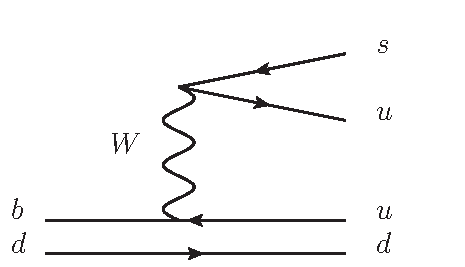
\includegraphics[width=\textwidth]{introduction/weak_tree}
    \caption{Tree diagram}
    \label{fig:intro:sm:weak_feynman:tree}
  \end{subfigure}
  \begin{subfigure}{0.55\textwidth}
    \centering
    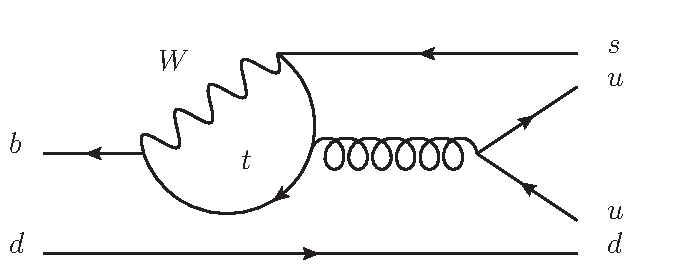
\includegraphics[width=\textwidth]{introduction/weak_penguin}
    \caption{Penguin diagram}
    \label{fig:intro:sm:weak_feynman:penguin}
  \end{subfigure}
  \caption{%
    Two possible Feynman diagrams for the decay \decay{\PBzero}{\PKplus\Ppiminus}.
  }
  \label{fig:intro:sm:weak_feynman}
\end{figure}
